\chapter{Game Design}\label{game design}
% collective action: a situation were it is denificial for agents to cooperate, inspite of their individual apirations. (ober 2008) common pool resource management, where each agent acts to maximise their own self interests, however, if all do this, the resource is depleated which defeats the long term goal of the gorup. lack of pro social behaviour acknowledgement and anti-social behaviour depleting resources. obedience and positive contribution is not directly percieved, but cost of defection is only fealt by those who will play in the long term. 

% computational justice: is the allocation fair? (what is meant by fair) 

% norm governed systems must deal with error, or defectors. 

% institutionlised power: agents empowered agents who can perform designated actions. agents in positions of power can identify and sanction defectors. 

% social choice theory: agregation of individual decisions or preferences to produce a single group decision.

% alternative dispute resolution: the resolution of any dispute between two or more entities that is resolved without the neeed for litigation. 

\section{Game Design}\label{sec: game design}

% Introduction to the game design section 
% What will be included in this chapter
This section will introduce the wide ranging mechanisms that allow agents to interact with collective action situations and perform different forms of knowledge aggregation. These coupled with the rules and regulations outlined in Section \ref{sec:rules}, will be embodied in a event flow diagram to illustrate the narrative of the game play. Finally, the algorithms that control the values of variables within the game will be presented, with the aim of fully educating the reader about every the aspect of the environment in which the agents live achieved by the end of this section. The mechanism are present as high-order logic only and should not be considered specific code implementations. These implementations will be detailed in Section. \ref{sec:infra}.


\subsection{Ideologies}\label{sec: ideologies}

% what do we wish to instill in the game. 
When considering self-organising multi-agent system, there are many different ideologies and scenarios that can be developed. When designing the game, the first decision was to create an economy of scarcity, meaning that the allocation of loot cannot satisfy all the agents individual desires. This condition sets the stage for Ostrom institutions to be formalised for achieving sustainment of the common pool resource. As a primary example, agents could be assigned access to the common pool based on a set of socially selected rules, or norms. Norm governed societies take into account not only the permissions and obligations of agents, but also the possibility that agents can deviate from the expected action. 

As knowledge aggregation is at the heart of all social interaction around a common goal, the design of the game considers social choice theory. The team wished to study how preference aggregation, possibly based upon facets such as an agent's reputation within the group, changes as the collective risk increases. Social choice theory is essentially the relationship between a collection of individual preferences and the final decision of the community. To keep the system as open as possible, the weighting of aggregation could be decided by the individual's definitions of contribution or utility, instead of a globally understood definition. This was regarded of paramount importance, as it allowed the analysis of different decision methods and how those methods influenced other agents. 

With regards to governance, granting institutionalised power to an agent who has been elected chair was considered to be an important mechanism for the formation of social contract proposals. Once passed, these rules represent the bedrock of an Ostrom institution. Introducing the concept of power implies the concept of fairness, or justice. Another important aspect was an agents content with the current chair's rule. For this, a mechanism for a divergence from the obliged action under a governing institution was created, coupled with a method of deposing chairs that do not conform to the agents ideals of fairness or equality. This can be extended to consider whether the allocation of resources was just. An interesting side note was the potential to identify and overthrow institutions that act according to their own interests, or the interest of an elitist clique. As with any defection from a social contract, this action can incur a sanction. In the interest of anarcho-socialism, these sanctions were deemed to be on a peer-to-peer basis and not at the institutionalised level. 

The survival game provides many different areas for social interaction for the formation of governments, proposals, collective actions and resource allocations. These will be introduced in the next section, with each mechanism attempting to embody the ideologies presented above. 

% What is our overall ideologies behind our design decisions
% introduce the following concepts
% social choice theory, collective action
% institutionalised power, norm governance and ADR. 
% computational justice 
% scalability

\section{Game Facets}\label{sec: game facets}

The identification of a number of different communication opportunities for agents to collectively self-organise through social interactions, allowed each goal to be compartmentalised into a separate collective action game. A collective action is defined as a situation where it is beneficial for agents to cooperate and act in the interest of the community, in spite of their individual aspirations \cite{ober2008}. This creation of conflicting agendas within agents can create some interesting situations, where an agent intent on maximising their own utility can harm the long term goal of the collective. However, pro-social behaviour is hard to identify. An agent's understanding of social capital can help to benefit a co-operational agent, especially in the presence of a negative sum game. This understanding can also serve to socially sanction anti-social behaviour where agents intentionally deplete resources, a cost that is only felt by those who will experience the game in the long term. Given the opportunity to create governments where the chair wields institutionalised power, agents elected to the chair empower other agents to vote on the proposals that have been granted access to the floor. The chair also is instilled with the power to assign permissions or obligations to members of the community, possibly based on concepts such as reputation or utility. Different interpretations of these socially agreed contracts allow agents to choose a path of obedience or disobedience, creating a framework for sanctions, forgiveness to inspire reconciliation and defiance to incite change \cite{pitt}.

This section will introduce the mechanisms used to allow agents to engage in these collective action discussions and arrive a decisions that endeavour to represent the collective good (according to what each agents definition of `good' is). The games will look to tackle issues such as Collective Risk Analysis, Common Pool Resource Allocation, Governance and Alternative Dispute Resolution by giving the agents methods of communication. This will allow a wide remit of knowledge aggregation methods, coupled with individual agent team's ideals of computational justice, social capital and collective utility. Finally, Social Choice Theory can combine all of these facets to produce decisions regarding the conditions for collective actions or individual actions. 
% short introduction those this sub section 
% collection action games

\subsection{Communication \& Discussion}\label{sec: comms}

% Basis of a Social Network 
% The heart of collection actions and preference aggregation
% Disstribution of Knowledge and Opinions DEFINITION
% knowledge aggregation
% Message Types and structures

At the heart of any social network is communication, discussion and information distribution. For this reason, an agent communication language must be developed to allow simple but meaningful interactions between agents that live in the environment. Many of the ideologies that have, to this point, been described require high amounts of knowledge aggregation to infer certain utility scores of social rankings. For this to be achieved, agents must be able to request information from each other such as; a combat opinion or social capital scores for other members of the community. These types of messages are considered informational and as such do not require a response. 

A different type of communication occurs at the institutional level. A chair has the ability to broadcast a proposal to all agents for a vote. This type of message is considered a request, and must be responded to immediately. However, the proposals themselves, common pool requests and obliged actions are one-way informational messages between the chair and the agents. 

The final type of communication occurs during peer-to-peer transactions. These message are also of request type and must be responded to. They were designed to follow the simple logic - `I offer X | I receive Y'. Gifts and straight swaps are allowed. 

The social network in the survival environment was defined to be fully connected. However, a limit to the number of messages relayed on any given round was imposed. The use of these message will be further detailed in the following section as and when they are used. 

\subsection{Governance}\label{sec: gov}

% Institutionalised Power
% Ostrom Institution Theory
% Alternate Disspute Resolution
% Computational Justice 
% Sanctions for dissobedience 
% Forgiveness

For the governance mechanism, chairs are elected based on a manifesto. The manifesto contains the conditions under which the running agent will rule. It contains the following points:

\begin{itemize}
    \item Term Length - No. of levels as chair,
    \item Deposal Threshold - \% no-confidence vote required to depose,
    \item Fight Decision Power - Power to alter fight proposal after a majority is agreed,
    \item Loot Decision Power - Power to allocate loot based on requests and an agreed proposal.
\end{itemize}

This election process happens at the end of each level, if the current chairs term has ended or if they are deposed. Any agent can run for office and a winner is elected via plurality (i.e. a relative majority). Once elected, for each level of their reign, there is a no-confidence vote after an enemy has been defeated. This forces the chair to consider a fair governance strategy if they wish to remain in power for the length of their term. 

While occupying the role of chair, the agent has the power to grant access to the floor so voting can take place regarding a proposal, be it for fight conditions or loot conditions. These proposals are determined by a pure majority. Once agreed, the chair has the responsibility to assign actions to members of the community based on these agreed social contracts. However, if they poses the power, the chair can alter the conditions of the contract after a majority is achieved. Obviously, this has implications for the stability of their rule and the communities individual implementations of computational justice. Other powers include the identification and labeling of defectors. 


\subsection{Fight Decisions}\label{sec: fight decision}

% Collective Risk Analysis
% Collective Action
% Social Contracts 
% Dissobedience 

The fight decision mechanism was designed to allow agents to perform collective risk analysis in a discussion based time period before each fight round. In this time, agents can gather information about their cohort, use different methods of computational aggregation and form individual preferences. The next stage required agents to submit proposals for the conditions under which each fight action is allocated based on the information and inferences gained from the collective risk analysis. The proposals should include thresholds for the following parameters and be determined for each action - attack, defend and cower. Agents are deemed suitable to fight if there attributes are above the required thresholds.  

\begin{itemize}
    \item $HP$
    \item $ST$
    \item Bonus Attack ($A_b$)
    \item Bonus Defense ($D_b$)
\end{itemize}

The chair proceeds to choose a proposal to present to the floor for a vote. If a majority is achieve, the social contract is implemented, otherwise the process is repeated. However, as introduced in Section \ref{sec: gov}, if the chair wields the Fight Decision Power, they may alter the conditions after a majority have been achieved. 

Finally, it is the responsibility of the chair to inform the community of their individual fight actions. Agents now have the choice of obedience (honor social contract) or disobedience (ignore obligation in favor of personal interests). After the fight round has completed, the chair can identify any defectors and release their names to the community for possible sanctions in the form of peer-to-peer trade embargos. Again, these sanctions are based on the individual agents definition of justice and the context of the defection. In some situations, having the bravery to defect under poor conditions could be be socially favourable. 

\subsection{Common Resource Allocation}\label{sec: cmr}

% Mechanism introudction 
% Dispute Resolution via Utility or Chair's ideology of fairness and agreed proposal
% Dissobediecence and thievery
% Sanctions and institutionalised power
% 
The loot allocation mechanism follows similar logic that of the fight decision. Agents have the opportunity to enter in discussions with the community to gather intelligence and inform future decisions. During this period, agents may also perform two tasks. Firstly, they may send requests to the chair for individual items of equipment within the loot common pool. Secondly, they may submit a proposal for the rules by which the loot is allocated. The proposals can include the same attribute thresholds as the fight decision proposals, and should state a rule for each type of equipment (i.e. sword, shield, health potion and stamina potion). After this period has elapsed, the chair, once again, selects a proposal and presents it to the floor for consideration. If a majority is achieved, then the rules of allocation are implemented in a social contact. However, if the chair wields the Loot Decision Power, they have the option of adjust the contract. 

Once a majority is achieved, the chair is responsible for allocating equipment to those agents who are eligible, due to the economy of scarcity, the majority of agents will receive no allocation. In the case of clashes in eligibility, the chair resolves these disputes using their own criteria, be it based on utility, social capital or some other metric. In should be noted that in the case the chair doesn't not wield the Loot Decision Power, the server resolves disputes and assigns equipment based on its internal metric of utility. 

The final stage of this mechanism gives agents access to the common pool resource in random order. Here agents have the opportunity to defect, and `steal' equipment that they are not eligible for. If this occurs, the chair can identify those involved and publicly share their identities for possible sanctions (as in Section. \ref{sec: fight decision}). 

This logic was chosen because it allows not only the chair to perform allocation based on its own ideologies, but also for agents to benefit greatly from defection (if they are lucky enough to be granted early access to the common pool). In this respect, the common resource allocation logic differs largely from the fight decision mechanism. 

\subsection{Peer-To-Peer Trading}\label{sec: trading}

% Individual analysis
% Social Capital 
% Fairness
% Clique Formation 

The final social interaction between the agents is the peer-to-peer trading. By design, this section was deliberately kept simple due to timing constraints. Agents can send requests to other members of the cohort, outlining the trade that they would like to complete. Gifts (Where something is given for nothing) can be done as well as straight swaps. Performing analysis on the frequency and density of these trades could reveal any strong social bonds between agents or the formation of cliques, where trades are restricted to only elite agents with the personal resources to trade. 

The trade requests detailed above are request type, therefore must be responded to immediately, therefore avoiding the acceptance of trades that are no longer viable. All trades that occur within the game are private and decentralised. 


\subsection{Public Vs. Private}\label{sec:pubpiv}

A small consideration was given the difference between publicly accessible attributes and privacy. The distinction was as follows:

\begin{itemize}
    \item Public:
    \begin{itemize}
        \item Enemy Resilience 
        \item Enemy Damage
        \item Agent Attributes ($HP$, $ST$, $A_b$, $D_b$)
    \end{itemize}
    \item Private:
    \begin{itemize}
        \item Inventory
        \item Internal Metrics (i.e. Social Capital)
    \end{itemize}
\end{itemize}

For the agent attributes $HP$ and $ST$, they will be highly granulated so that agents cannot know specific levels of health or stamina. This should introduce some uncertainty into calculations and therefore increase the non-determinism of the game. 

\subsection{Utility \& Defining A Winner}\label{sec: winner}

% Relative average contribution w.r.t a number of facets
% ideology surrounding a `winner' of a fight
% ethics surronunding selfishness and sacrifice 
Finally, a winner of the game had to be defined. This proved to be one of the harder tasks because, as will all collective action games, the survivor with the most hit-points doesn't entail being the most contributive to the community. Other aspects of ethics and philosophy were also considered. Take, as an example, an agent who intentionally sacrifices themselves so that the collective can advance. How is this action scored? For this reason, a global utility score was derived according to a number of facets. In each respect, the average over the whole community is taken and agents are assigned points based on their deviations from these averages (above incurs an increase, below a decrease in utility). The facets are listed in the following enumeration. It should be noted that facets with a * proceeding it indicate that the score is inverse. 

\begin{enumerate}
    \item $HP$ remaining
    \item $ST$ remaining
    \item $A_b$
    \item $D_b$
    \item Total $HP_{pool}$ donations 
    \item No. of Attack decisions
    \item No. of Defence decisions
    \item No. of Cower decisions * 
    \item No. of trades completed
    \item No. of items left in inventory *
\end{enumerate}

As the scored are based on a collective average, these individual facets are equally weighted. For the purposes of analysis, this utility score can be calculated for sub-samples-sets including individual agents, separate agent types and the whole cohort. The objective is to observe if certain agent strategies lend themselves to one of more of the above facets (with respect to the collective). 


\subsection{Agent Consideration \& Possible Behaviour}\label{sec: behaviour}

% possible behaviour
% possible traits to consider
% i.e social capital, contribution, effectivness, dissobedience
% Personal utility 

For integration with the facets described above, each agent must consider at minimum the following traits:

\begin{itemize}
    \item Social Capital
    \item Contribution
    \item Effectiveness
    \item Disobedience 
\end{itemize}

Each of these areas are separate mechanisms of knowledge aggregation and can be used to inform decisions about combat, leadership and socially trusted networks. The individual algorithmic definitions of these traits are considered private and therefore can only be known though social interaction. The choice to have independent agents with possibly conflicting intuitions of these traits was intentional. It is the hope that during analysis, different interpretations of the traits will show different levels of bias towards the self or the collective. 


\subsection{Game Flow}\label{sec:game flow}

Now that the many different aspects of the game have been introduced, Figure \ref{fig:game flow} shows the overall flow of the game. It is clear to see that the game is split into two different loops, a nested fight round and the overarching level loop. 

\begin{figure}[htb]
    \centering
    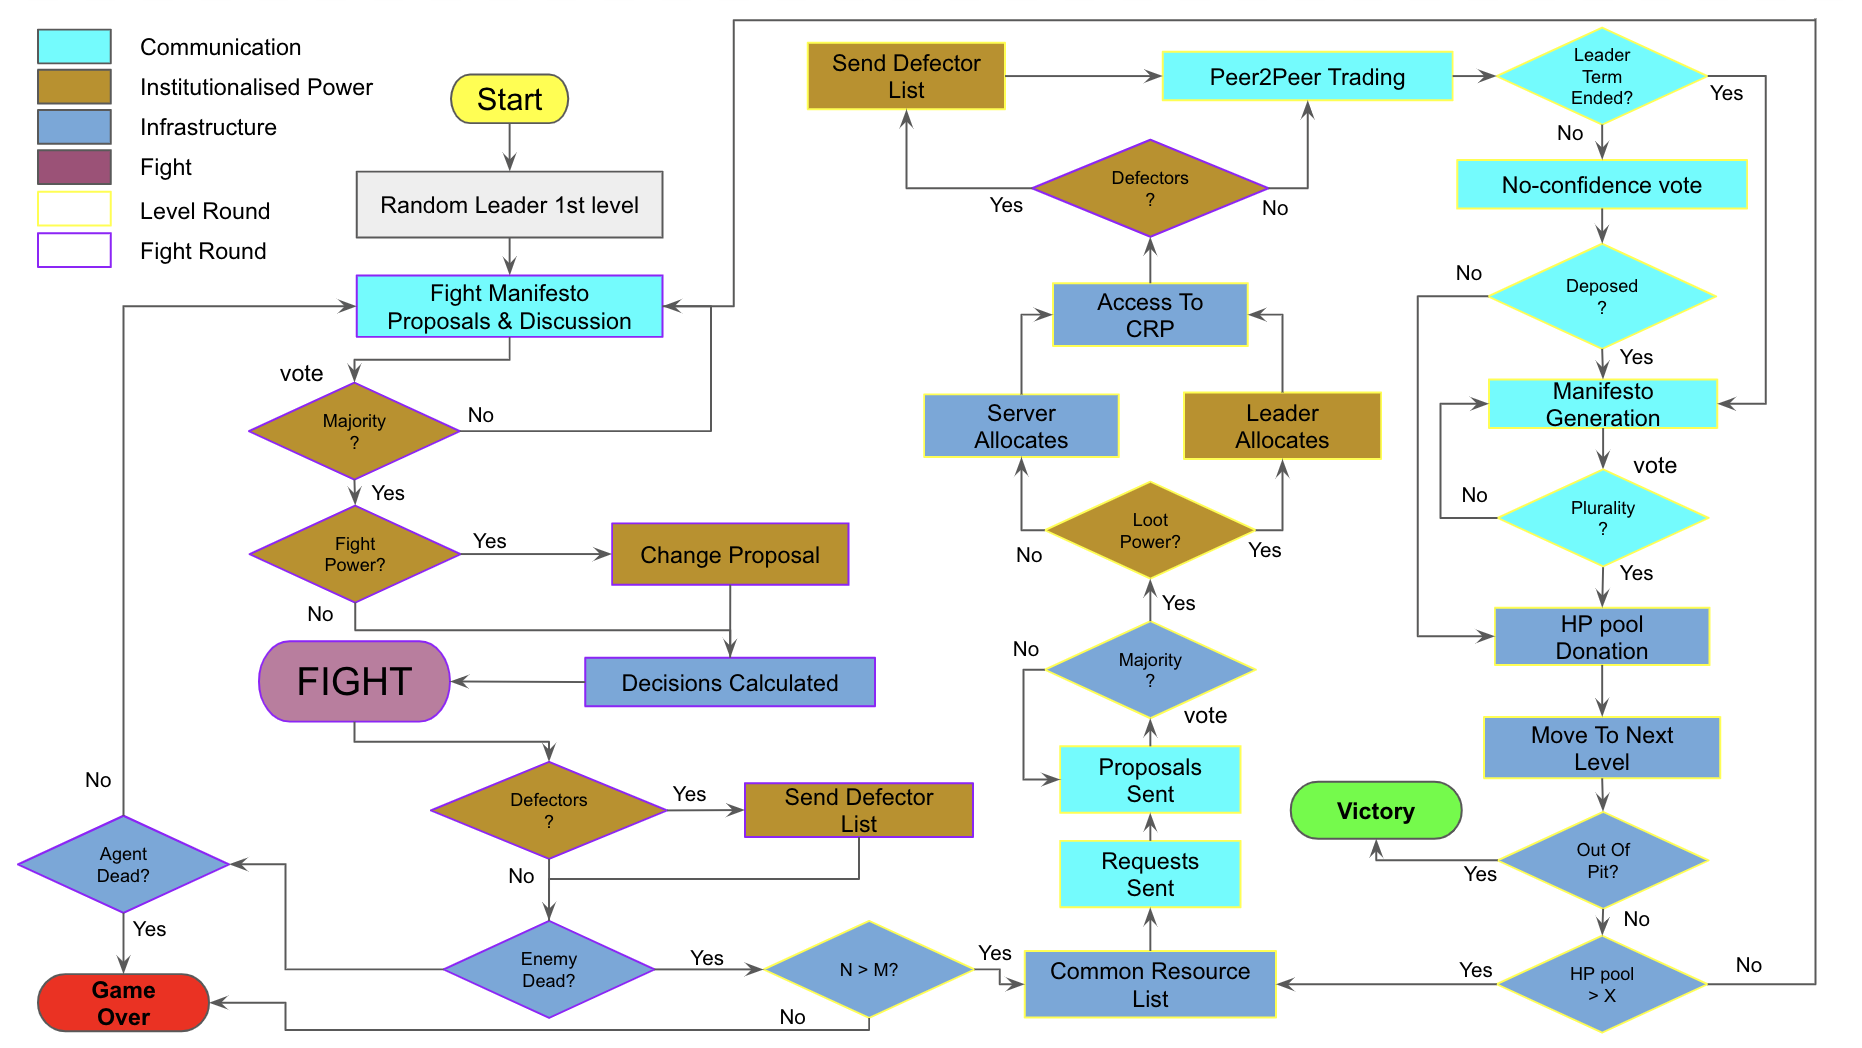
\includegraphics[scale=0.5]{001_game_design/images/gameflow.png}
    \caption{Flow Chart Of The Cooperative Survival Game To Experiment The Pit}
    \label{fig:game flow}
\end{figure}

\section{Mathematics}\label{sec: maths}

In this sub-section, the variables of the game are defined using dynamic algorithms and initial instantiations. All equations are designed so that the difficulty of the game is invariant to initial conditions. This way, only the self-organisational abilities of different numbers of agents determines the effectiveness of the strategy. 

For increasingly difficult game play, the enemy attributes were designed to be of increasing in value, linearly, over the duration of the game. To introduce non-determinism, each calculation should be randomly scaled within a pre-determined range, and each use of an attack weapon only deal a percentage range of it maximum potential. The frequency of equipment dropped by defeated enemies was designed to force an economy of scarcity, where in not all agents can be satisfied by the allocation of the common resource pool (loot). With regards to individual pieces of loot, values are directly proportional to the strength of the enemy defeated. Therefore, as the game gets increasingly more difficult, the equipment available to the agents becomes increasingly more powerful.  

Finally, the metric used for calculating the utility of an agent with respect to the group will be introduced as an indicator of the winner of the game. Each agent will be scored based on their relative contribution compared with the average over the course of the game. 

\subsection{Initial Variables}\label{sec: initial variable}

For decent game play with a single agent from each team (i.e. 6 agents), and assuming that integer values of all variables are preferable for readability for logging, the stating values are assigned as below. 

\begin{itemize}
    \item Health Points - $HP = 1000$
    \item Stamina - $ST = 2000$
    \item Number of Agents - $N = 100$
    \item Number of Levels - $L = 60$
    \item Threshold Percentage - $\mu = 0.6$
\end{itemize}

Here the Threshold Percentage, is the percentage of agents ($N$) required to be alive at the end of the game to win, as shown in Equation \ref{eq:M}. All of these starting variables can be adjusted, and will dynamically scale the other variables within the game to ensure consistency of difficulty. 

\begin{equation}\label{eq:M}
    M = ceil(\mu N)
\end{equation}

There are some variables within the game that are dependent on `$HP_{start}$'. This variable represents the starting value, not the current value. For this reason, $HP/ST/N/L$ initial values should be globally defined. The $ceil()$ function is to ensure integer values. It can be implemented in whatever way is best. To satisfy rule 9, the following two equations define the amount of health/stamina that the action of cowering regenerates.  
% Agents starting attributes and infra strating values 

\begin{equation}
    HP_c = 0.01*HP_{start}
\end{equation}

\begin{equation}
    ST_c = 0.01*HP_{start}
\end{equation}


\subsection{Modifiers}\label{sec: modifiers}

% hit points and range modifiers
% non-detminism introduction 

For the introduction of non-determinism, two modifiers were created. The first, $\delta$, is a range modifier that ensures each calculated value falls within a plus-minus range. This range was determined to be $20\%$, so the range modifier has the bounds, $0.8 \leq \delta \leq 1.2 $, and is shown in Equation \ref{eq:delta}. This modifier will be used in all the equations throughout the game. 

\begin{equation}\label{eq:delta}
    \delta = random(0.8,1.2)
\end{equation}

The second is the hit-point modifier, $\gamma$. This ensures that any damage dealt during an attack action, by either the enemy or an agent, only deals a percentage of it's maximum hit potential. $\gamma$ has the bounds, $0.5 \leq \lambda \leq 1$ and can be seen in Equation \ref{eq:gamma}. 

\begin{equation}\label{eq:gamma}
    \gamma = random(0.5,1)
\end{equation}


\subsection{Enemy Variables}\label{sec: enemy}

% equation representation and the reasons for this 
% i.e. Monster resiliance is base on HP and ST the caluclate the minimum monster resilience ove the whole game for a winnable situtation whilst also making the game difficulty invarient over starting parameters. 

Enemy variables are designed to create the same difficulty regardless of the starting values to assess the effectiveness of the self-organisation of different numbers of agents. The first enemy attribute is the resiliance ($X$), and is shown in Equation \ref{eq:X}. This was deisgned to be a ratio of total amount of combined damage that all the agents are capable of, based on their starting stamina value, and the number of levels in the game. This ensures that, overall, the game is just winnable and easily loosable given high thresholds of surviving agents and/or poor self-organisation. 

\begin{equation}\label{eq:X}
    X = ceil \left( \delta \frac{N(ST)}{L} \sigma \right)
\end{equation}

Where $\sigma$ is the linear scaling variable defined as:

\begin{equation}
    \sigma = \frac{2c}{L} + 0.5
\end{equation}

with $c$ representing the current level of the pit. $\sigma$ is used to linearly scale the monster's resilience as the players traverse the levels of the pit. Changing this equation (i.e. to an exponential form) will change the distribution with which the monsters get stronger, around the average resilience. Increasing the difficulty of the game is easily done by modifying $\sigma$.

The second, and final, enemy attribute is the monster's damage rating ($Y$), and can be seen in Equation \ref{eq:Y}. It was design with similar logic to the enemy's resilience. That is, the ratio of the total potential health and shield points of all the agents against the number of levels is considered, ensuring that the enemy can deal enough damage to kill the required number of agents so that the group fails its obective. To ensure this, the ratio is scaled by 1 minus the threshold percentage.  

\begin{equation}\label{eq:Y}
    Y = ceil \left(\delta \frac{N(HP)+N(ST)}{L} \sigma \left(1-\frac{M}{N} \right) \right)
\end{equation}

Where $\delta$ and $\sigma$ the same as for $X$. As outlined eariler in this section, each time the monster attacks, its hit points are a percentage of its total potential $Y$. Therefore, the instantaneous values of $Y$ becomes:

\begin{equation}
    Y_{hit points} = \gamma Y 
\end{equation}


\subsection{Loot Variables} \label{sec: loot}

% Introduction to Loot
% Quantity Equation Definitions
% Quality Equation Definitions 
As a quick reminder, every time a monster is defeated, it drops a number of equipment (weapons/shields) and a number of potions (health/stamina), these represent the `loot' or common pool. As outlined in Section \ref{introduction}, every agent has a base value and a bonus value of attack and defence. Each agent starts with a base Attack ($D_s$), and Defense ($S_s$) with the values $0.005*ST$. The base value represents an agents minimum potential.
Bonus Attack ($A_b$) and Bonus Defence ($D_b$) is dictated by the equipment currently being wielded. Within each fight round, each agent who chooses to fight, deals a percentage of either $D_b$ or $A_b$, depending on their chosen fight action. This is defined as the $\gamma$ modifier outlined in Section \ref{sec: modifiers}. After use, the resulting hit-value is subtracted from the agents stamina ($ST$), meaning that an agent's stamina degrades with every use of equipment. For Potions, the value of any given potion, when consumed, is added to the agents $HP$ (for health potions) or $ST$ (for stamina potions). 

This sub-section will introduce the equations used for calculating both the value of all equipment and the frequency with which these are dropped. 


% Each equipment gets dropped by the monster once defeated. 
% Each agent starts with base case - fists/skin.

\subsubsection{Loot Drop Frequency}

New equipment is created at the end of each level, after enemy disposal. The number of equipment/potions dropped per monster is determined by the number of agents that started the game. The range modifier, $\delta$ is used to further add non-determinisium to the loot mechanism. For the number of potions dropped,

\begin{equation}
    N_p = \delta P N
\end{equation}

where $0 \leq P \leq 1$ and is predetermined in order to create an economy of scarcity. The number of equipment dropped is,

\begin{equation}
    N_e = \delta E N
\end{equation}

where $0 \leq E \leq 1$ and is also predetermined (i.e. $P=0.2$, $E=0.15$). 

% each equipment is created at each new level. 
% the monster drops:
% Potions (Np) as a percentage of the number of agents 
% Equipment (Ne) as a percentage of the number of agents (Np<Ne)

\noindent For both potions and equipment, there are two different pieces to drop. For potions, the number of health potions dropped is,

\begin{equation}
    P_{hp} = \tau N_p
\end{equation}

and stamina potions,

\begin{equation}
    P_{st} = (1-\tau) N_p
\end{equation}

where $\tau$ is,

\begin{equation}
    \tau = random(0,1).
\end{equation}

\noindent The same logic applies of the equipment drop. The number of weapons,

\begin{equation}
    N_w = \tau N_e
\end{equation}

and the number of shields,

\begin{equation}
    N_s = (1 - \tau) N_e. 
\end{equation}

$\tau$ is re-calculated for equipment so that the split between the two variables is not the same. 
% within these:
% Weapons dropped (Nw) is a random percentage of Ne
% Shields dropped (Ns) is (1-random_number) of Ne

% Health Potions dropped (Php) is a random percentage of Np
% Stamina Potions dropped (Pst) is (1-random_number) of Np

\subsubsection{Loot Values}

For the value of the these potions and equipment, they are dependent on the attributes of the monster that was just defeated. Dropped weapon damage ($D_i$) is a percentage of ($X_i$),

\begin{equation}
    D_i = ceil\left (\delta \frac{X_i}{4N(0.8)} \right)
\end{equation}

\noindent Dropped shield protection ($S_i$) is a percentage of ($Y_i$),

\begin{equation}
    S_i = ceil \left( \delta \frac{Y_i}{N(0.8)}0.5 \right)
\end{equation}

and the same applies for the potions. Health as,

\begin{equation}
    P_h = ceil \left( \delta \frac{Y_i}{N(0.8)}5 \right)
\end{equation}

and stamina,

\begin{equation}
    P_s = ceil \left( \delta \frac{X_i}{N(0.8)} \right)
\end{equation}

\noindent The only issue with this, is that the increase of the values over the levels is bounded to the increase of $X$ and $Y$.

